%============================
% SECTION 6: SLICE RENDERING
%============================
\section{Interactive Slice Rendering}

\begin{frame}
\frametitle{Textured Quad Rendering}

\textbf{Approach:} Render 2D slice as textured quad in 3D space

\begin{center}
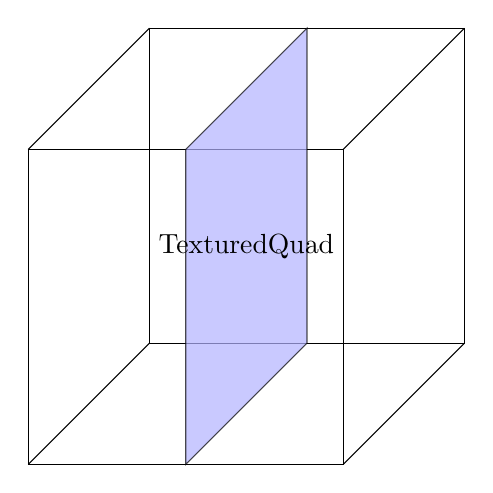
\begin{tikzpicture}[scale=2]
  % 3D volume
  \draw (0,0,0) -- (2,0,0) -- (2,2,0) -- (0,2,0) -- cycle;
  \draw (0,0,2) -- (2,0,2) -- (2,2,2) -- (0,2,2) -- cycle;
  \draw (0,0,0) -- (0,0,2);
  \draw (2,0,0) -- (2,0,2);
  \draw (2,2,0) -- (2,2,2);
  \draw (0,2,0) -- (0,2,2);
  
  % Textured quad
  \draw[fill=blue!30, opacity=0.7] (1,0,0) -- (1,2,0) -- (1,2,2) -- (1,0,2) -- cycle;
  \node at (1, 1, 1) {Textured\\Quad};
\end{tikzpicture}
\end{center}

\begin{itemize}
  \item Extract 2D slice from volume
  \item Create texture from slice data
  \item Position quad in 3D space (perpendicular to axis)
  \item Apply texture and render
\end{itemize}
\end{frame}

\begin{frame}[fragile]
\frametitle{Slice Texture Update}

\begin{lstlisting}
updateSliceTextureFromVolume(
  axis: 'axial' | 'sagittal' | 'coronal',
  index: number
) {
  // Extract 2D slice from volume
  const slice = this.volume.getSliceUint8(axis, index);
  
  // Create or update texture
  if (!this.sliceTexture) {
    this.sliceTexture = this.gl.createTexture();
  }
  
  this.gl.bindTexture(this.gl.TEXTURE_2D, this.sliceTexture);
  
  // Upload slice data as texture
  this.gl.texImage2D(
    this.gl.TEXTURE_2D, 0, this.gl.LUMINANCE,
    slice.width, slice.height, 0,
    this.gl.LUMINANCE, this.gl.UNSIGNED_BYTE,
    slice.data
  );
  
  // Set texture parameters
  this.gl.texParameteri(this.gl.TEXTURE_2D, 
    this.gl.TEXTURE_MIN_FILTER, this.gl.LINEAR);
  this.gl.texParameteri(this.gl.TEXTURE_2D, 
    this.gl.TEXTURE_MAG_FILTER, this.gl.LINEAR);
}
\end{lstlisting}
\end{frame}

\begin{frame}[fragile]
\frametitle{Quad Geometry Creation}

\begin{lstlisting}
updateSliceMesh(axis: 'axial' | 'sagittal' | 'coronal', 
                index: number) {
  
  let positions: number[] = [];
  let texcoords: number[] = [];
  
  if (axis === 'axial') {
    // Quad at z = index, spans x and y
    const z = this.indexToWorldZ(index);
    const minX = 0, maxX = 1;
    const minY = 0, maxY = 1;
    
    positions = [
      minX, minY, z,  // bottom-left
      maxX, minY, z,  // bottom-right
      minX, maxY, z,  // top-left
      maxX, maxY, z   // top-right
    ];
    
    texcoords = [
      0, 0,  // UV mapping
      1, 0,
      0, 1,
      1, 1
    ];
  }
  // Similar for sagittal and coronal...
  
  // Update GPU buffers
  this.updateGeometryBuffers(positions, texcoords);
}
\end{lstlisting}
\end{frame}

\begin{frame}
\frametitle{Real-time Interaction}

\textbf{Slice Selection via Widgets:}

\begin{center}
\includegraphics[width=0.9\textwidth]{../assets/slice-control.png}
\end{center}

\begin{itemize}
  \item Slider for axial index: 0 to depth-1
  \item Slider for sagittal index: 0 to width-1
  \item Slider for coronal index: 0 to height-1
  \item onChange: Update slice texture and geometry
  \item Immediate visual feedback
\end{itemize}
\end{frame}

\begin{frame}
\frametitle{Bounding Box Visualization}

\textbf{Purpose:} Show volume extent in 3D space

\begin{itemize}
  \item Render wireframe box around volume
  \item Helps spatial understanding
  \item Simple line geometry (8 vertices, 12 edges)
  \item Uses separate shader program
\end{itemize}

\vspace{0.5cm}

\textbf{Box Coordinates:}
\begin{itemize}
  \item Min corner: $(0, 0, 0)$
  \item Max corner: $(W, H, D)$ (scaled by spacing)
  \item Normalized to $[0, 1]^3$ for rendering
\end{itemize}

\vspace{0.5cm}

\textbf{Rendering:}
\begin{itemize}
  \item Separate shader program (simpleVert/simpleFrag)
  \item Line primitive: \texttt{gl.LINE\_LOOP}
  \item Fixed color (e.g., white outline)
\end{itemize}
\end{frame}

